\documentclass[tikz, border=2mm]{standalone}
\usepackage{tikz}

\begin{document}


    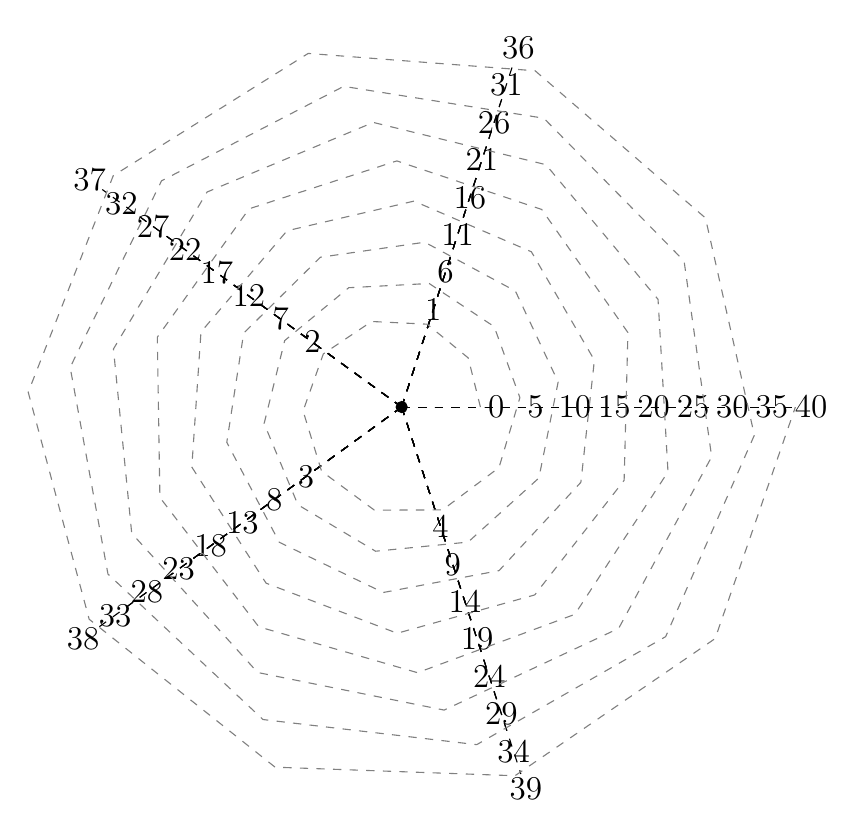
\begin{tikzpicture}

        % Define parameters
        \def\n{5}           % Number of sections per full turn (mod 7)
        \def\maxnum{40}      % Maximum number to display
        \def\start_radius{1} % Starting radius
        \def\gap{0.5}        % Radial growth per step
        \def\angle{360/\n}   % Angle step per section

        % Draw the spiral wheel
        \foreach \k in {0,...,\maxnum} {
            % Compute angular position smoothly, winding outward
            \pgfmathsetmacro{\theta}{(\k) * \angle} % Angle increases with each number

            % Compute radial distance smoothly increasing
            \pgfmathsetmacro{\newradius}{\start_radius + \k * \gap / \n}

            % Draw connecting radial lines for structure
            \draw[dashed] (0,0) -- (\theta:\newradius);

            % Place number labels in the spiral
            \node[font=\large] at (\theta:\newradius + 0.2) {\k};
        }

        % Draw a smooth spiral guide (optional, helps visualization)
        \draw[thin, dashed, gray, domain=0:360*\maxnum/\n, samples=\maxnum*2]
            plot ({(1 + \gap * \x / 360) * cos(\x)}, {(1 + \gap * \x / 360) * sin(\x)});

        % Mark the center
        \filldraw[black] (0,0) circle (2pt);

    \end{tikzpicture}


\end{document}